% Source: quantum_distribution_functions.pdf, pages 1-9 (page 10 is blank). Title on the source:
% "Quantum distribution functions and applications, including superconductivity, superfluidity,
% Bose-Einstein condensation in dilute atomic vapors". No lecture number.
\subsection{Quantum distribution functions}
\subsubsection*{Fermions, bosons and the grand canonical ensemble}

Particles with half-integral spin in units of $\hbar$, denoted fermions, are subject to the Pauli Exclusion Principle,
which forbids two identical fermions from occupying the same quantum state. Pauli inferred this from the observed fact that
as the number of electrons in an atom increases (with $N_e = N_p$ in neutral atoms), these electrons do not go into the
lowest-energy orbital, but instead occupy progressively higher orbitals: H: $(1s)^1$ ($\uparrow$), He: $(1s)^2$
($\uparrow\downarrow$), Li: $(1s)^2(2s)^1$ ($\uparrow\downarrow$, $\uparrow$), etc. The Pauli Exclusion Principle is
embodied in the requirement that the quantum-mechanical wavefunction for fermions is antisymmetric under the interchange of
two identical fermions:
\begin{equation}
  \psi(\ldots(\mathbf x_i,\mathbf s_i)\ldots(\mathbf x_j,\mathbf s_j)\ldots) = -\psi(\ldots(\mathbf x_j,\mathbf s_j)\ldots(\mathbf x_i,\mathbf s_i)\ldots).
\end{equation}
Particles with integral spins (bosons) have wavefunctions that are symmetric under interchange of identical bosons:
\begin{equation}
  \psi(\ldots(\mathbf x_i,\mathbf s_i)\ldots(\mathbf x_j,\mathbf s_j)\ldots) = \psi(\ldots(\mathbf x_j,\mathbf s_j)\ldots(\mathbf x_i,\mathbf s_i)\ldots).
\end{equation}

We have dealt with systems with a fixed number of particles (e.g.\ atoms/molecules in a gas or spins at sites of a lattice)
and for these one uses the canonical ensemble (partition function) $Z = \sum_{\text{states}}e^{-\beta\Ham}$. A natural
generalization for systems with variable numbers of particles is the grand canonical ensemble:
\begin{equation}
  Z_G = \sum_re^{\alpha n_r}\cdot e^{-\beta\Ham} = \sum_re^{-\beta(E_r^{\text{tot.}}-\mu n_r)},
\end{equation}
where $\beta = 1/(\kB T)$, $\alpha\equiv\beta\mu$ and $\mu$ = ``chemical potential''; $\Omega_G = -\kB T\ln Z_G$, so
\begin{equation}
  \ev n = \frac{\sum_rn_re^{-\beta(E_r^{\text{tot}}-\mu n_r)}}{\sum_re^{-\beta(E_r^{\text{tot}}-\mu n_r)}}
        = \frac{1}{\beta}\frac{\partial\ln Z_G}{\partial\mu} = \frac{\partial\ln Z_G}{\partial\alpha}.
\end{equation}
For a system with $n_r$ fermions in a quantum state with energy $E_r$, the total energy is $E_r^{\text{tot}} = n_rE_r$.

\subsubsection*{The Fermi--Dirac distribution}

So we can write (for fermions)
\begin{equation}
  \sum_{n_r}e^{-\beta(E_r^{\text{tot}}-\mu n_r)} = \sum_{n_r=0}^1e^{-\beta n_r(E_r-\mu)} = 1 + e^{-\beta(E_r-\mu)},
\end{equation}
so $\ln Z_G = \sum_r\ln\left(1+e^{-\beta(E_r-\mu)}\right)$ and
\begin{equation}
  \ev n = \sum_r\ev{n_r} = \frac{1}{\beta}\frac{\partial\ln Z_G}{\partial\mu}
  = \sum_r\frac{e^{-\beta(E_r-\mu)}}{1+e^{-\beta(E_r-\mu)}} = \sum_r\frac{1}{e^{\beta(E_r-\mu)}+1}
\end{equation}
\begin{equation}
  \Rightarrow\quad\boxed{\ev{n_r} = \frac{1}{e^{\beta(E_r-\mu)}+1}}.
\end{equation}
This is the \emph{Fermi--Dirac} (quantum) distribution function. As $T\to 0$, i.e.\ $\beta\to\infty$:
\begin{equation}
  \ev{n_r} = \begin{cases}\dfrac{1}{e^{-\infty}+1} = 1 & \text{if } E_r<\mu\\[6pt] \dfrac{1}{e^{\infty}+1} = 0 & \text{if } E_r>\mu .\end{cases}
\end{equation}
Here, $\mu$ is called the ``Fermi energy'' and, at $T = 0$, all states with energies $E_r<\mu$ are occupied, while all
states with energies $E_r>\mu$ are unoccupied. At a finite temperature $T$, if $E_r = \mu$, then $\ev{n_r} = 1/2$.

\begin{diagram}
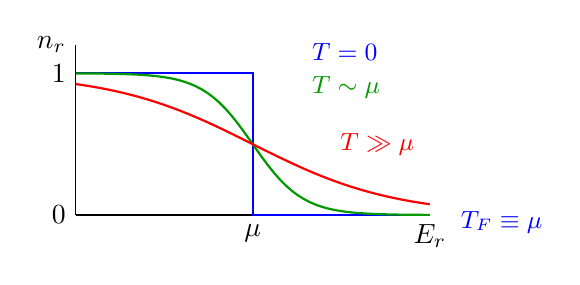
\begin{tikzpicture}[scale=0.9]
  \draw (0,0) -- (5,0) node[below] {$E_r$}; \draw (0,0) -- (0,2.4) node[left] {$\ev{n_r}$};
  \draw[thick,blue] (0,2) -- (2.5,2) -- (2.5,0) -- (5,0);
  \draw[thick,green!60!black,domain=0:5,samples=60] plot (\x,{2/(exp((\x-2.5)/0.35)+1)});
  \draw[thick,red,domain=0:5,samples=60] plot (\x,{2/(exp((\x-2.5)/1.0)+1)});
  \node[left] at (0,2) {$1$}; \node[left] at (0,0) {$0$}; \node[below] at (2.5,0) {$\mu$};
  \node[blue,font=\small,anchor=west] at (3.2,2.3) {$\kB T = 0$};
  \node[green!60!black,font=\small,anchor=west] at (3.2,1.8) {$\kB T\sim\mu$};
  \node[red,font=\small,anchor=west] at (3.6,1.0) {$\kB T\gg\mu$};
  \node[blue,font=\small,anchor=west] at (5.3,-0.1) {$\kB T_F\equiv\mu$};
\end{tikzpicture}
\diagramcaption{The Fermi--Dirac distribution.}
\end{diagram}

We will use this distribution later to study some properties of electrons in metals. A typical Fermi energy for electrons
in a metal is $\mu\sim\text{eV}\sim\kB\cdot(10^4$--$10^5\ \text{K})$. So ambient temperatures, $27^\circ\text{C}\simeq 300$~K,
are $\ll T_F\sim 10^4$--$10^5$~K. This means that the electrons fill the ``Fermi sea'' of states with $E_r\le\mu$. Note that
the green and red curves are theoretical; a typical metal can melt and vaporize before the temperature reaches $T_F$; e.g.\
$T_F(\text{Cu}) = 8.12\times 10^4\ \text{K}>T_{\text{boil}}(\text{Cu}) = 2.84\times 10^3$~K;
$T_F(\text{Al}) = 1.35\times 10^5\ \text{K}>T_{\text{boil}}(\text{Al}) = 2.74\times 10^3$~K.

\subsubsection*{The Bose--Einstein distribution}

Next, consider bosons; for these, with $x = e^{-\beta(E_r-\mu)}$,
\begin{equation}
  \sum_{n_r=0}^\infty e^{-\beta n_r(E_r-\mu)} = \sum_{n_r=0}^\infty x^{n_r} = \frac{1}{1-x} = \left[1-e^{-\beta(E_r-\mu)}\right]^{-1},
\end{equation}
\begin{equation}
  Z_G = \sum_{\text{states}}\sum_{n_r=0}^\infty e^{-\beta n_1(E_1-\mu)-\beta n_2(E_2-\mu)\cdots}
      = \prod_r\frac{1}{1-e^{-\beta(E_r-\mu)}},
\end{equation}
so
\begin{equation}
  \ln Z_G = -\sum_r\ln\left[1-e^{-\beta(E_r-\mu)}\right],
\end{equation}
\begin{equation}
  \ev n = \frac{1}{\beta}\frac{\partial\ln Z_G}{\partial\mu} = -\sum_r(-1)\left[\frac{e^{-\beta(E_r-\mu)}}{1-e^{-\beta(E_r-\mu)}}\right]
        = \sum_r\frac{1}{e^{\beta(E_r-\mu)}-1},
\end{equation}
so
\begin{equation}
  \boxed{\ev{n_r} = \frac{1}{e^{\beta(E_r-\mu)}-1}},
\end{equation}
the \emph{Bose--Einstein} distribution function (Satyendra Bose, A.~Einstein, 1924).

For these distribution functions, $\mu\to-\mu$ for particle $\to$ antiparticle, so since photons (which have spin 1 and
hence are bosons) are self-conjugate, $\mu_\gamma = 0$ and $\ev{n_r} = 1/(e^{\beta E_r}-1)$ for photons.

\subsection{Superconductivity and superfluidity}
\subsubsection*{Superconductivity}

The phenomenon of Bose--Einstein condensation (BEC) was inferred by Bose and Einstein from the BE distribution function. It
is the basic physics responsible for superconductivity and superfluidity. It was first observed in simple systems of dilute
atomic vapors in 1995. Recall some basics.

Superconductivity (SC). An electric current $I$ flowing through a conductor with a resistance $R$ has ohmic power
dissipation $P = I^2R$. For a wire of area $A$, length $\ell$, $R = \rho\ell/A$, where $\rho$ = resistivity
($\rho = 1/\sigma$, where $\sigma$ = conductivity). Metals are distinguished from insulators by the presence of
(quasi)free electrons in the conduction band. The resistivity of a metal is due to the inelastic scattering of the e's in a
current from other e's, dissipating energy. As the temperature is reduced, the resistivity $\rho$ decreases. In 1911,
Kamerlingh Onnes (working in Leiden) discovered that when certain metals were cooled to temperatures below a few K, $\rho$
abruptly vanished, and when a voltage difference was applied, the resultant electric current would flow without any measurable
resistance. The critical temperatures at which this superconductivity transition occurs are:
\begin{gather*}
  T_c = 7.19\ \text{K for Pb (lead)},\qquad T_c = 4.15\ \text{K for Hg (mercury)},\\
  T_c = 3.7\ \text{K for Sn (tin)},\qquad T_c = 9.25\ \text{K for Nb (niobium)}.
\end{gather*}
For this far-reaching discovery, Onnes received the Nobel Prize in 1913. Phenomenological theories of superconductivity were
developed in the 1920s--1940s (London, Landau and Ginzburg, \ldots). In 1957, Bardeen, Cooper, and Schrieffer (BCS) presented
a microscopic theory of superconductivity, for which they received the Nobel Prize in 1972. According to the BCS theory, the
superconductivity is due to the attractive electron--proton interaction, manifested as an electron--phonon interaction, where
phonons are quantized lattice vibrations; in turn, this leads to an electron pairing into ``Cooper pairs'', $\ev{ee}$. These
are bosonic quasiparticles and undergo Bose--Einstein condensation, with macroscopic occupation number in the ground state.
Because there is a finite energy gap between the ground state and excited states, when electrons flow as part of an electric
current, they cannot undergo an inelastic scattering, since there is insufficient energy to reach an excited state. The flow of
electrons is thus free of energy dissipation, i.e.\ the resistivity is zero.

In 1986, another important advance was made when Georg Bednorz and K.~Alex M\"uller (at IBM Z\"urich) discovered
``high-temperature superconductivity'' (HTSC), namely SC with $T_c\sim 30$~K in LaBa$_2$Cu$_3$O$_{7-x}$ (``LBCO'',
lanthanum--barium--copper oxide). For this discovery, Bednorz and M\"uller received the 1987 Nobel Prize. Subsequently,
researchers found HTSC with $T_c\sim 90$~K in YBa$_2$Cu$_3$O$_{7-x}$ (``YBCO'', yttrium--barium--copper oxide). This was notable
because when $T_c>77$~K, the experiments can use liquid N$_2$ with $T_\ell = 77$~K for cooling, rather than liquid He. Intensive
theoretical and experimental effort has gone into the study of HTSC since 1986. Because the HTSC compounds are brittle, they
have not been applied very much in engineering. Superconductivity has also been observed in stacked layers of graphene.

$\ev{ee}$ carries charge $-2$, so the Cooper pair condensate effectively breaks $U(1)_{em}$; the photon gets an effective mass,
$m_\gamma^2\propto ne^2/m_e$, which leads to the Meissner Effect: in contrast to the situation with a normal metal,
which allows a nonzero magnetic field in its interior, a superconductor excludes a magnetic field:
\begin{equation}
  \mathbf B(x)\sim|\mathbf B(0)|e^{-x/\lambda_L},
\end{equation}
where $x$ is the distance into the superconductor and $\lambda_L = 1/m_\gamma$ is the ``London penetration depth''; a
typical value is $\lambda_L\sim 5\times 10^2\ \text{\AA} = 50$~nm. Some SC (type II SC) allow a $\mathbf B$ field to penetrate,
but only in filaments. These have been used for magnetic resonance imaging (MRI) machines for medical imaging, which have
$\mathbf B$ fields of order 2--4 Tesla. They have also been crucial for wiring to carry high electrical currents in magnets to
bend protons and antiprotons in high-energy particle colliders ($\mathbf F = q\mathbf v\times\mathbf B$); e.g.\ Nb$_3$Sn has
$T_c = 18.3$~K and can take current densities $\sim 2\times 10^3$~Amps/mm$^2$ at $|\mathbf B|\sim 4$~T at $T\sim 4.1$~K. The
FNAL $\bar pp$ Tevatron Collider used NbTi, with $T_c\sim 10$~K and $J\sim 2\times 10^3$~Amp/mm$^2$ at $|\mathbf B|\sim 4.5$~T,
and this was also used at $T = 1.9$~K, $|\mathbf B| = 8.3$~T at the Large Hadron ($pp$) Collider LHC. These enabled very large
currents with very low overall power dissipation. (See the note added at the end.)

\subsubsection*{Superfluidity}

Superfluidity: a superfluid flows without any viscosity. The viscosity in a normal fluid is analogous to the resistivity of a
metal; the viscosity is due to the particles in the fluid undergoing inelastic collisions and dissipating energy, just as the
resistivity of the metal is due to the electrons in the electric current undergoing inelastic collisions and dissipating energy.
For a fluid composed of bosons, e.g.\ liquid He ($^4_2$He = $(ppnn)$ nucleus $+$ 2 e's, total spin 0), at sufficiently low
temperature, a macroscopic number of atoms can undergo Bose--Einstein condensation, going into the ground state. Because there is
an energy gap separating this from excited states, the bosons cannot scatter and go into higher-energy states, so the flow is
dissipationless.

The phenomenon of superfluidity (SF) was discovered by P.~Kapitsa in 1937, in his experiments on liquid He; for this, Kapitsa
received the Nobel Prize in 1978. Landau focused much of his research on superfluidity and it was for this work that he
received the 1962 Nobel Prize. Recall the phase diagram for He (Lecture 4): in addition to the 1st-order phase boundaries
separating the gas, normal fluid, and solid phases, He has a line (really curve), the ``$\lambda$-line'' of 2nd-order phase
transitions separating the normal fluid and superfluid phases; $p_c = 2.25$~atm, $T_c = 5.195$~K, $T_\ell = 4.22$~K,
$(T_c)_\lambda = 2.177$~K at $p = 1$~atm, and the triple point at 2.18~K and $p\simeq 0.05$~atm.

The Bose--Einstein condensation underlying superconductivity and superfluidity involves relatively strongly interacting systems
(solid metal, liquid He). For many decades, physicists tried to achieve BEC in a much simpler system, namely a dilute atomic
vapor. In 1995, this was achieved: W.~Ketterle et al.\ observed BEC in a dilute vapor of $^{23}_{11}$Na atoms at MIT, and
E.~Cornell and C.~Wieman et al.\ observed BEC in a dilute vapor of $^{87}_{37}$Rb atoms at U.~Colorado--JILA (Joint Inst.\ for
Lab.\ Astroph.)--NIST. For this discovery these three researchers received the Nobel Prize in 2001. Now let us analyze the
phenomenon of BEC.

\subsection{Bose--Einstein condensation}
\subsubsection*{When are quantum coherence effects important?}

We begin with a general analysis of when quantum coherence effects are important. The criterion for this is that the
interparticle spacing $R\lesssim\lambda\!\!\!^-$, where $\lambda\!\!\!^- = \hbar/p$ is the de Broglie wavelength (divided
by $2\pi$; $\lambda\!\!\!^- = \lambda/(2\pi)$) of the relevant particles. For a gas of $N$ particles occupying a volume $V$
in $d$ dimensions ($d = 3$ here), the average volume occupied by each particle is $v = V/N$ and $v = R^d$, so
$R = \left(V/N\right)^{1/d}$. For a gas at $p\sim 1$~atm and room temperature $T\sim 300$~K, the ideal gas EOS is a very good description
and so $pV = N\kB T$, $p/(\kB T) = N/V = \rho_n$, so $R = \left(V/N\right)^{1/d} = \left(\kB T/p\right)^{1/d}$. The kinetic
energy of a gas particle is $E_{\text{kin.}} = |\mathbf p|^2/(2m) = d\cdot\kB T/2$, by the equipartition theorem, so
$|\mathbf p|\equiv p = \sqrt{d\cdot m\kB T}$, and the de Broglie wavelength is
\begin{equation}
  \lambda\!\!\!^- = \frac{\hbar}{p} = \frac{\hbar}{\sqrt{d\cdot m\kB T}},
\end{equation}
so the conditions under which quantum mechanical effects will be important are $R\lesssim\lambda\!\!\!^-$, i.e.
\begin{equation}
  \left(\frac{V}{N}\right)^{1/d}\lesssim\frac{\hbar}{\sqrt{d\cdot m\kB T}}.
\end{equation}
Recall that for a gas at $p\sim 1$~atm and $T\sim 300$~K, $R\sim 34\ \text{\AA} = 3.4$~nm. And
\begin{equation}
  \lambda\!\!\!^- = \frac{\hbar}{\sqrt{3m\kB T}} = \frac{N_A\hbar}{\sqrt{3MRT}},
\end{equation}
where, e.g., for N$_2$ (with $^{14}_7$N), $M = 28$~g/mole $= N_Am$, and $R = N_A\kB = 8.314$~J/(mole$\cdot$K), so
\begin{equation}
  \lambda\!\!\!^- = \frac{(6.02\times 10^{23}\ \text{mol}^{-1})(1.05\times 10^{-34}\ \text{J}\cdot\text{sec})}{\left[3(0.028\ \text{kg})\left(8.314\ \frac{\text{J}}{\text{mol}\cdot\text{K}}\right)(300\ \text{K})\right]^{1/2}}
  = 4.3\times 10^{-12}\ \text{m} = 4.3\times 10^{-3}\ \text{nm}.
\end{equation}
So $R\sim 10^3\lambda\!\!\!^-$ in this gas.

Of course, as we discussed before, the very existence of atoms and molecules is due to quantum mechanics: a classical electron in
the Coulombic electric field of a nucleus is not in a stable state; it is accelerated in its orbit around the nucleus and hence
radiates electromagnetic waves, losing energy and spiraling in to the nucleus. So what is meant here is that
$R\lesssim\lambda\!\!\!^-$ leads to observable quantum coherence effects. This condition $\lambda\!\!\!^-\gtrsim R$ is, for
$d = 3$:
\begin{equation}
  \frac{\hbar}{[3m\kB T]^{1/2}}\gtrsim\left(\frac{V}{N}\right)^{1/3},\quad\text{i.e.}\quad
  \frac{\hbar^2}{3m\kB T}\gtrsim\left(\frac{V}{N}\right)^{2/3},\quad\text{i.e.}\quad
  \boxed{\frac{\hbar^2}{3m}\left(\frac{N}{V}\right)^{2/3}\gtrsim\kB T}.
\end{equation}
So high density and low temperature $\Rightarrow\lambda\!\!\!^-\gtrsim R$. This rough estimate will be seen to have the same
functional form, $\kB T_c\sim(\text{no.})(\hbar^2/m)\left(N/V\right)^{2/3}$, as the actual Bose--Einstein condensation
temperature; they only differ in the numerical coefficient.

\subsubsection*{The condensation temperature}

The total number of bosons, $N$, can be divided into the number in the ground state (g.s.) and the number in excited states:
\begin{equation}
  N = N_0 + \sum_{\text{excited states }r}n_r = N_0 + \sum_{\text{excited states }r}\frac{1}{e^{\beta(E_r-\mu)}-1}.
\end{equation}
The excited states may be approximated as closely spaced (although the gap with the g.s.\ is retained), so replace the sum by an
integral, $\dd N = L^3\dd^3k/(2\pi)^3$, where $L^3$ is the volume. So
\begin{equation}
  N = N_0 + g_J\left(\frac{L}{2\pi}\right)^3\int\frac{\dd^3k}{e^{\beta(E_k-\mu)}-1},
\end{equation}
where $g_J = 2J+1$ is the statistical factor, with $J$ = spin. With $\dd^3k = 4\pi k^2\dd k$ and
$k^2\dd k = k\cdot(k\,\dd k) = k\cdot(1/2)\dd k^2$,
\begin{align}
  \int\frac{\dd^3k}{(\cdots)} &= 4\pi\int_0^{k_{\max}}\frac{k^2\dd k}{(\cdots)} = 2\pi\int_0^{k_{\max}}\frac{k\,\dd k^2}{(\cdots)}\nonumber\\
  &= \frac{2\pi}{\hbar^3}\int_0^{p_{\max}}\frac{p\,\dd p^2}{(\cdots)} = \frac{2\pi}{\hbar^3}(2m)^{3/2}\int\frac{\sqrt E\,\dd E}{(e^{\beta(E-\mu)}-1)},
\end{align}
where now $p = \hbar k$, and $E = p^2/(2m)$, so $p = \sqrt{2mE}$. Because of the exponential decrease of the integrand as $E$
gets large, we can extend the range of integration to $\infty$, obtaining the result
\begin{equation}
  N = N_0 + g_J\left(\frac{L}{2\pi\hbar}\right)^3\cdot 2\pi(2m)^{3/2}\underbrace{\int_0^\infty\frac{E^{1/2}\dd E}{(e^{\beta(E-\mu)}-1)}}_{\beta^{-3/2}\int_0^\infty x^{1/2}\dd x/(e^{x-\beta\mu}-1)},
\end{equation}
where we define a dimensionless variable $x = \beta E = E/(\kB T)$. It is convenient to re-express this in terms of
$N/V = \rho_n$, the number density, where $V = L^3$:
\begin{equation}
  \left(\frac{N}{V}\right) = \left(\frac{N_0}{V}\right) + \underbrace{\frac{g_J}{(2\pi)^2}\left(\frac{2m\kB T}{\hbar^2}\right)^{3/2}\int_0^\infty\frac{x^{1/2}\dd x}{(e^{x-\beta\mu}-1)}}_{N_{\text{excited}}/V}.
\end{equation}
Consider a situation in which a large number of particles are in the $E = 0$ state, so
\begin{equation}
  N = \frac{1}{e^{\beta(E-\mu)}-1} = \frac{1}{e^{-\beta\mu}-1};\quad\text{expand}\ \to\ \frac{1}{(1-\beta\mu\ldots)-1} = -\frac{1}{\beta\mu} = -\frac{\kB T}{\mu},
\end{equation}
so $\mu\simeq-\kB T/N\to 0$ in this case. So we can approximate the integral as
\begin{equation}
  \int_0^\infty\frac{x^{1/2}\dd x}{e^x-1} = \frac{\sqrt\pi}{2}\zeta(3/2),
\end{equation}
where $\zeta(s) = \sum_{n=1}^\infty(1/n^s)$ is the Riemann zeta function and $\zeta(3/2) = 2.61238\ldots$. So at the
temperature where there is just beginning to be a significant $N_0$, we have
\begin{equation}
  \left(\frac{N_{\text{excited}}}{V}\right) = \left(\frac{g_J}{4\pi^2}\right)\left(\frac{2m\kB T_c}{\hbar^2}\right)^{3/2}\frac{\sqrt\pi}{2}\zeta(3/2)
  = \frac{g_J}{8}\left(\frac{2m\kB T_c}{\pi\hbar^2}\right)^{3/2}\zeta(3/2).
\end{equation}
So as $T\to T_c^+$, $N_{\text{excited}}\simeq N$, so, solving for $T_c$:
\begin{gather}
  \frac{N_{\text{excited}}}{V}\simeq\frac{N}{V} = \frac{g_J}{8}\left(\frac{2m\kB T_c}{\pi\hbar^2}\right)^{3/2}\zeta(3/2)
  \ \Rightarrow\ \left(\frac{8N}{g_J\zeta(3/2)V}\right)^{2/3} = \frac{2m\kB T_c}{\pi\hbar^2}\nonumber\\
  \Rightarrow\quad\boxed{\kB T_c = \frac{2\pi\hbar^2}{m}\left(\frac{N}{g_J\zeta(3/2)V}\right)^{2/3}},
\end{gather}
the BEC condensation temperature (see, e.g., Kittel, \emph{Thermal Physics}). Numerically,
\begin{equation}
  \kB T_c = 3.31\frac{\hbar^2}{m}\left(\frac{\rho_n}{g_J}\right)^{2/3}.
\end{equation}

As an illustrative calculation for the experimental conditions of the MIT group, consider their dilute atomic vapor of Na
($^{23}_{11}$Na) atoms. They achieved $\rho_n\simeq 1.5\times 10^{14}$~cm$^{-3}$:
\begin{equation}
  T_c = \frac{3.31(1.054\times 10^{-34}\ \text{J}\cdot\text{s})^2(1.5\times 10^{20}\ \text{m}^{-3})^{2/3}}{g_J^{2/3}(1.38\times 10^{-23}\ \text{J/K})(23)(1.67\times 10^{-27}\ \text{kg})}
  = \frac{2.0\times 10^{-6}\ \text{K}}{g_J^{2/3}};
\end{equation}
see PRL \textbf{75}, 3969 (1995) for the MIT result (several $J$ values are mentioned).

Since $N_{\text{exc}}/V\propto T^{3/2}$ and $N/V\propto T_c^{3/2}$ with the same proportionality constant,
$N_{\text{exc}}/N = \left(T/T_c\right)^{3/2}$, so
\begin{equation}
  N_0 = N - N_{\text{exc}} = N\left(1-\frac{N_{\text{exc}}}{N}\right) = N\left[1-\left(\frac{T}{T_c}\right)^{3/2}\right].
\end{equation}

\begin{diagram}
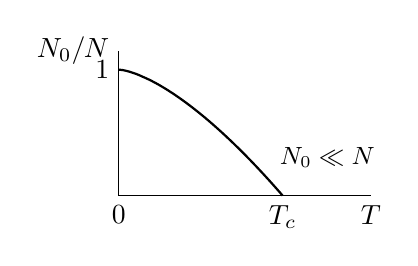
\begin{tikzpicture}[scale=0.8]
  \draw (0,0) -- (4,0) node[below] {$T$}; \draw (0,0) -- (0,2.3) node[left] {$N_0/N$};
  \draw[thick,domain=0:2.6,samples=50] plot (\x,{2*(1-(\x/2.6)^1.5)});
  \node[left] at (0,2) {$1$}; \node[below] at (0,0) {$0$}; \node[below] at (2.6,0) {$T_c$};
  \node[font=\small,anchor=west] at (2.4,0.6) {$N_0\ll N$};
\end{tikzpicture}
\diagramcaption{The condensate fraction below $T_c$.}
\end{diagram}

This calculation applies reasonably accurately for the dilute vapors of the type used by the MIT, Colorado--JILA--NIST, and other
groups, and also, approximately, to the BEC in the normal--superfluid phase transition in liquid He. Near the $\lambda$ line at
$p = 1$~atm, the (mass) density of the liquid He is $\rho\simeq 0.14$~g/cm$^3$. Converting this to the number density and
substituting in the equation for $T_c$, one gets $T_c\sim 3$~K, which is close to the experimentally observed $T_c = 2.177$~K.

As discussed before, both the superconducting and the superfluid phase transitions are of the 3D $U(1) = O(2)$ universality class,
since the Cooper pair condensate and the superfluid wavefunction have phases $e^{\ii\theta}\sim U(1)$.

\paragraph{Note added on recent research on high-\texorpdfstring{$T_c$}{Tc} superconductivity.}

Since the discovery of the HTSCs by Bednorz and M\"uller in 1987, there has been intensive research on many materials in order to
develop HTSCs with higher $T_c$. One direction of recent research has been to test materials under high-pressure conditions.
Recall the conversion relations: $1\ \text{atm} = 1\ \text{bar} = 101\ \text{kPa} = 0.1$~MPa;
$1\ \text{kbar} = 10^3\ \text{atm} = 100$~MPa; $10\ \text{kbar} = 10^4\ \text{atm} = 1$~GPa;
$1\ \text{Mbar} = 10^6\ \text{atm} = 100$~GPa, where Pa = Newton/meter$^2$. See tables of $T_c(p)$ values for various substances
from reviews on HTSCs. A key milestone was the discovery of HTSCs with $T_c>T_\ell(\text{N}_2) = 77$~K; these could be studied
rather easily using liquid N$_2$ as a coolant, instead of the more expensive liquid He. In the late 1980s, this was achieved, e.g.\
with BiSrCaCuO, TlBaCaCuO, HgBaCaCuO, with $T_c$ up to $\sim 140$~K. Work on developing high-$T_c$ materials has continued.
